\documentclass[12pt, a4paper, oneside]{article}
\usepackage{amsmath, amsthm, amssymb, bm, graphicx, hyperref, mathrsfs, multirow, booktabs, array, circuitikz, karnaugh-map, tikz}
\usetikzlibrary{circuits.logic.IEC,automata}
\usetikzlibrary{shapes,arrows,calc,arrows.meta}
\ctikzset{logic ports=ieee}
\tikzset{d-ff/.style={flipflop, flipflop def={
    t1=C, t3=D, t4=Q}}
}
\tikzset{d-ff1/.style={flipflop, flipflop def={
    t1=D, t3=C, t4={\ctikztextnot{Q}},t6=Q}}
}
\tikzset{t-ff/.style={flipflop, flipflop def={
    t1=C, t3=T, t4=Q}}
}

\title{\textbf{Assignment\#4 CS207 Fall 2023}}
\author{Ben Chen(12212231)}
\date{\today}
\linespread{1.43}
\newcounter{problemname}
\newenvironment{problem}{\stepcounter{problemname}\par\noindent\textsc{Problem \arabic{problemname}. }}{\\\par}
\newenvironment{solution}{\par\noindent\textsc{Solution. }}{\\\par}
\newenvironment{note}{\par\noindent\textsc{Note of Problem \arabic{problemname}. }}{\\\par}

\begin{document}

\maketitle

\begin{problem}
    Given the function table, design a 4-bit register with four DFF and 4X1 MUX whose mode selection inputs are $S_1$ and $S_0$.
\end{problem}

\begin{solution}
    According to the description of operations, we can derive the function table as follows
    \begin{table}[!htbp]
    \caption{Function Table of 4-bit Register}
    \centering
    \begin{tabular}{p{.09\textwidth}<{\centering}p{.09\textwidth}<{\centering}p{.09\textwidth}<{\centering}p{.09\textwidth}<{\centering}p{.09\textwidth}<{\centering}p{.09\textwidth}<{\centering}p{.2\textwidth}<{\centering}}
        \toprule
        \multicolumn{2}{c}{\textbf{Mode}} & \multicolumn{4}{c}{\textbf{Output}} & Register \\
        \cmidrule(lr){1-2}\cmidrule(lr){3-6}\cmidrule(lr){7-7}
        $S_1$ & $S_0$ & $A_3$ & $A_2$ & $A_1$ & $A_0$ & Operation \\
        \midrule
        0 & 0 & $A_3$ & $A_2$ & $A_1$ & $A_0$ & No change \\
        0 & 1 & $A_3^{\prime}$ & $A_2^{\prime}$ & $A_1^{\prime}$ & $A_0^{\prime}$ & Complement \\
        1 & 0 & 0 & 0 & 0 & 0 & Reset \\
        1 & 1 & $I_3$ & $I_2$ & $I_1$ & $I_0$ & Load Parallel \\
        \bottomrule
    \end{tabular}
    \end{table}
    \newline And to design the circuit, we first connect the input wires to the port 3 of each multiplexer to load the data in parallel,
    and then connect the $s_0$ to the port 2 of each multiplexer to have the register reset,
    and put the output wire back to the port 1 with inverter to get the complement and port 0 to have the register unchanged of each multiplexer.
    \begin{figure}[!htbp]
        \centering
        \setlength{\belowcaptionskip}{+0.4cm}
        \begin{circuitikz}[circuit logic IEC]
            \draw (-0.3,4cm) node[d-ff, rotate=90] (dff1) {};
            \draw (3.2cm,4cm) node[d-ff, rotate=90] (dff2) {};
            \draw (6.7cm,4cm) node[d-ff, rotate=90] (dff3) {};
            \draw (10.2,4cm) node[d-ff, rotate=90] (dff4) {};
            \draw (0,0) node[and gate, inputs={nn}, and gate IEC symbol={}, text height=1.7cm,text width=1.7cm, very thick] (A) {};
            \draw (3.5cm,0) node[and gate, inputs={nn}, and gate IEC symbol={}, text height=1.7cm,text width=1.7cm, very thick] (B) {};
            \draw (7cm,0) node[and gate, inputs={nn}, and gate IEC symbol={}, text height=1.7cm,text width=1.7cm, very thick] (C) {};
            \draw (10.5cm,0) node[and gate, inputs={nn}, and gate IEC symbol={}, text height=1.7cm,text width=1.7cm, very thick] (D) {};
            \draw ([xshift=-0.7cm]A.input 1) node[left] {$s_1$} -- (A.input 1);
            \draw ([xshift=-0.7cm]A.input 2) node[left] {$s_0$} -- ++(0.3cm,0) node[fill=black,shape=circle,scale=0.3] (sn0) {} -- (A.input 2);
            \draw (dff1.pin 4) -- ++(0,0.1cm) node[fill=black,shape=circle,scale=0.3] (qn1) {} -- ++(0,0.7cm) node[above] {$A_3$};
            \draw (dff2.pin 4) -- ++(0,0.1cm) node[fill=black,shape=circle,scale=0.3] (qn2) {} -- ++(0,0.7cm) node[above] {$A_2$};
            \draw (dff3.pin 4) -- ++(0,0.1cm) node[fill=black,shape=circle,scale=0.3] (qn3) {} -- ++(0,0.7cm) node[above] {$A_1$};
            \draw (dff4.pin 4) -- ++(0,0.1cm) node[fill=black,shape=circle,scale=0.3] (qn4) {} -- ++(0,0.7cm) node[above] {$A_0$};
            \draw ( $ (A.south west)!0.20!(A.south east) $ ) -- ++(-90:0.25) |- ++(0,5pt) node[above] {$3$};
            \draw ( $ (A.south west)!0.40!(A.south east) $ ) -- ++(-90:0.25) |- ++(0,5pt) node[above] {$2$};
            \draw ( $ (A.south west)!0.60!(A.south east) $ ) -- ++(-90:0.25) |- ++(0,5pt) node[above] {$1$};
            \draw ( $ (A.south west)!0.80!(A.south east) $ ) -- ++(-90:0.25) |- ++(0,5pt) node[above] {$0$};
            \draw ( $ (B.south west)!0.20!(B.south east) $ ) -- ++(-90:0.25) |- ++(0,5pt) node[above] {$3$};
            \draw ( $ (B.south west)!0.40!(B.south east) $ ) -- ++(-90:0.25) |- ++(0,5pt) node[above] {$2$};
            \draw ( $ (B.south west)!0.60!(B.south east) $ ) -- ++(-90:0.25) |- ++(0,5pt) node[above] {$1$};
            \draw ( $ (B.south west)!0.80!(B.south east) $ ) -- ++(-90:0.25) |- ++(0,5pt) node[above] {$0$};
            \draw ( $ (C.south west)!0.20!(C.south east) $ ) -- ++(-90:0.25) |- ++(0,5pt) node[above] {$3$};
            \draw ( $ (C.south west)!0.40!(C.south east) $ ) -- ++(-90:0.25) |- ++(0,5pt) node[above] {$2$};
            \draw ( $ (C.south west)!0.60!(C.south east) $ ) -- ++(-90:0.25) |- ++(0,5pt) node[above] {$1$};
            \draw ( $ (C.south west)!0.80!(C.south east) $ ) -- ++(-90:0.25) |- ++(0,5pt) node[above] {$0$};
            \draw ( $ (D.south west)!0.20!(D.south east) $ ) -- ++(-90:0.25) |- ++(0,5pt) node[above] {$3$};
            \draw ( $ (D.south west)!0.40!(D.south east) $ ) -- ++(-90:0.25) |- ++(0,5pt) node[above] {$2$};
            \draw ( $ (D.south west)!0.60!(D.south east) $ ) -- ++(-90:0.25) |- ++(0,5pt) node[above] {$1$};
            \draw ( $ (D.south west)!0.80!(D.south east) $ ) -- ++(-90:0.25) |- ++(0,5pt) node[above] {$0$};
            \draw ( $ (A.south west)!0.20!(A.south east) $ ) -- ++(-90:0.25) |- ++(0,-1.8cm) node[below] {$I_3$};
            \draw ( $ (A.south west)!0.40!(A.south east) $ ) -- ++(-90:0.25) |- ++(0,-1.3cm) node[fill=black,shape=circle,scale=0.3] (sn1) {};
            \draw ( $ (A.south west)!0.60!(A.south east) $ ) -- ++(-90:0.25) |- ++(0,5pt) node[notcirc] {} -- ++(0,-1cm) -- ++(1.3cm,0) |- (qn1);
            \draw ( $ (A.south west)!0.80!(A.south east) $ ) -- ++(-90:0.25) |- ++(0,5pt) -- ++(0,-1cm) node[fill=black,shape=circle,scale=0.3] {};
            \draw ( $ (B.south west)!0.20!(B.south east) $ ) -- ++(-90:0.25) |- ++(0,-1.8cm) node[below] {$I_2$};
            \draw ( $ (B.south west)!0.40!(B.south east) $ ) -- ++(-90:0.25) |- ++(0,-1.3cm) node[fill=black,shape=circle,scale=0.3] (sn2) {};
            \draw ( $ (B.south west)!0.60!(B.south east) $ ) -- ++(-90:0.25) |- ++(0,5pt) node[notcirc] {} -- ++(0,-1cm) -- ++(1.3cm,0) |- (qn2);
            \draw ( $ (B.south west)!0.80!(B.south east) $ ) -- ++(-90:0.25) |- ++(0,5pt) -- ++(0,-1cm) node[fill=black,shape=circle,scale=0.3] {};
            \draw ( $ (C.south west)!0.20!(C.south east) $ ) -- ++(-90:0.25) |- ++(0,-1.8cm) node[below] {$I_1$};
            \draw ( $ (C.south west)!0.40!(C.south east) $ ) -- ++(-90:0.25) |- ++(0,-1.3cm) node[fill=black,shape=circle,scale=0.3] (sn3) {};
            \draw ( $ (C.south west)!0.60!(C.south east) $ ) -- ++(-90:0.25) |- ++(0,5pt) node[notcirc] {} -- ++(0,-1cm) -- ++(1.3cm,0) |- (qn3);
            \draw ( $ (C.south west)!0.80!(C.south east) $ ) -- ++(-90:0.25) |- ++(0,5pt) -- ++(0,-1cm) node[fill=black,shape=circle,scale=0.3] {};
            \draw ( $ (D.south west)!0.20!(D.south east) $ ) -- ++(-90:0.25) |- ++(0,-1.8cm) node[below] {$I_0$};
            \draw ( $ (D.south west)!0.40!(D.south east) $ ) -- ++(-90:0.25) |- ++(0,-1.3cm) node[above] (sn4) {};
            \draw ( $ (D.south west)!0.60!(D.south east) $ ) -- ++(-90:0.25) |- ++(0,5pt) node[notcirc] {} -- ++(0,-1cm) -- ++(1.3cm,0) |- (qn4);
            \draw ( $ (D.south west)!0.80!(D.south east) $ ) -- ++(-90:0.25) |- ++(0,5pt) -- ++(0,-1cm) node[fill=black,shape=circle,scale=0.3] {};
            \draw[thin] ( $ (A.north west)!.8!(A.north east) $ ) node[below] {$y$} -| (dff1.pin 3);
            \draw[thin] ( $ (B.north west)!.8!(B.north east) $ ) node[below] {$y$} -| (dff2.pin 3);
            \draw[thin] ( $ (C.north west)!.8!(C.north east) $ ) node[below] {$y$} -| (dff3.pin 3);
            \draw[thin] ( $ (D.north west)!.8!(D.north east) $ ) node[below] {$y$} -| (dff4.pin 3);
            \draw (dff1.pin 1) -- ++(0,-0.5cm) node[fill=black,shape=circle,scale=0.3] (clkn1) {} ;
            \draw (dff2.pin 1) -- ++(0,-0.5cm) node[fill=black,shape=circle,scale=0.3] (clkn2) {} ;
            \draw (dff3.pin 1) -- ++(0,-0.5cm) node[fill=black,shape=circle,scale=0.3] (clkn3) {} ;
            \draw (dff4.pin 1) -- ++(0,-0.5cm) -- (clkn3) -- (clkn2) -- (clkn1) -- ++(-0.5cm,0) node[left] {$clk$};
            \draw[-{Latex[length=2mm]}] ([xshift=1.9cm]A.input 1) node {} -- (B.input 1);
            \draw[-{Latex[length=2mm]}] ([xshift=1.9cm]A.input 2) node {} -- (B.input 2);
            \draw[-{Latex[length=2mm]}] ([xshift=1.9cm]B.input 1) node {} -- (C.input 1);
            \draw[-{Latex[length=2mm]}] ([xshift=1.9cm]B.input 2) node {} -- (C.input 2);
            \draw[-{Latex[length=2mm]}] ([xshift=1.9cm]C.input 1) node {} -- (D.input 1);
            \draw[-{Latex[length=2mm]}] ([xshift=1.9cm]C.input 2) node {} -- (D.input 2);
            \draw (sn0) |- (sn1) -- (sn2) -- (sn3) -| (sn4);
        \end{circuitikz}
    \end{figure}
\end{solution}

\begin{problem}
    Design a sequence generator to generate the sequence 1011110.
\end{problem}

\begin{solution}
    The bit length is 7, so we need 4 \textit{DFF}s since 3 \textit{DFF}s will lead to duplicate state. And we can derive the state table as follows
    \begin{table}[!htbp]
        \centering
        \begin{tabular}{|p{.13\textwidth}<{\centering}|p{.13\textwidth}<{\centering}|p{.13\textwidth}<{\centering}|p{.13\textwidth}<{\centering}|p{.13\textwidth}<{\centering}|p{.13\textwidth}<{\centering}|}
        \hline
        CLK & $Z$ & $Q_3$ & $Q_2$ & $Q_1$ & $Q_0$ \\ \hline
        $\uparrow$ & 0 & 1 & 0 & 1 & 1 \\ \hline
        $\uparrow$ & 1 & 0 & 1 & 0 & 1 \\ \hline
        $\uparrow$ & 1 & 1 & 0 & 1 & 0 \\ \hline
        $\uparrow$ & 1 & 1 & 1 & 0 & 1 \\ \hline
        $\uparrow$ & 1 & 1 & 1 & 1 & 0 \\ \hline
        $\uparrow$ & 0 & 1 & 1 & 1 & 1 \\ \hline
        $\uparrow$ & 1 & 0 & 1 & 1 & 1 \\ \hline
        \end{tabular}
    \end{table}
    \newline And we can derive the Karnaugh map as follows
    \begin{table}[!htbp]
        \centering
        \begin{karnaugh-map}(label=corner)[4][4][1][$Q_0$][$Q_1$][$Q_2$][$Q_3$]
            \minterms{5,7,10,13,14}
            \terms{11,15}{0}
            \autoterms[X]
            \implicantedge{0}{8}{2}{10}
            \implicant{0}{9}
            \implicant{0}{6}
        \end{karnaugh-map}
    \end{table}
    \newline so we can derive the simplified equations as follows
    \[ Z = Q_3^{\prime} + Q_1^{\prime} + Q_0^{\prime} \]
    And the logic diagram will be
    \begin{figure}[!htbp]
        \centering
        \setlength{\belowcaptionskip}{+0.4cm}
        \begin{circuitikz}[circuit logic IEC]
            \draw (0,0) node[d-ff1] (dff1) {};
            \draw (3cm,0) node[d-ff1] (dff2) {};
            \draw (6cm,0) node[d-ff1] (dff3) {};
            \draw (9cm,0) node[d-ff1] (dff4) {};
            \draw (0, -3cm) node[or port, number inputs=3, rotate=180] (or) {};
            \draw (dff1.pin 3) -- ++(0,-0.5cm) -- ++(0,-0.5cm) node[above] (clkn1) {} ;
            \draw (dff2.pin 3) -- ++(0,-0.5cm) -- ++(0,-0.5cm) node[fill=black,shape=circle,scale=0.3] (clkn2) {} ;
            \draw (dff3.pin 3) -- ++(0,-0.5cm) -- ++(0,-0.5cm) node[fill=black,shape=circle,scale=0.3] (clkn3) {} ;
            \draw (dff4.pin 3) -- ++(0,-0.5cm) -- ++(0,-0.5cm) node[yshift=-3pt, below] {$clk$} -- (clkn3) -- (clkn2) -| (clkn1);
            \draw (dff1.pin 4) -- ++(5pt,0) |- (or.in 3)
                  (dff3.pin 4) -- ++(5pt,0) |- (or.in 2)
                  (dff4.pin 4) -- ++(5pt,0) |- (or.in 1);
            \draw (dff1.pin 6) -- (dff2.pin 1)
                  (dff2.pin 6) -- (dff3.pin 1)
                  (dff3.pin 6) -- (dff4.pin 1);
            \draw (dff1.pin 1) -- ++(-10pt,0) node[left] {$Z$} |- (or.out) -- ++(-0.39cm,0) node[fill=black,shape=circle,scale=0.3] {} -- ++(-1cm,0) node[above] {output};
        \end{circuitikz}
    \end{figure}
\end{solution}

\begin{problem}
    Design a synchronous counter using DFFs that has the following sequence:
    \[ 0010, 0110, 1001, 1000, 1100, 1101 \] 
    From the undesired states the counter must go back on the next clock pulse.
\end{problem}

\begin{solution}
    From the sequence, we can derive the state diagram as follows
    \begin{figure}[!htbp]
        \centering
        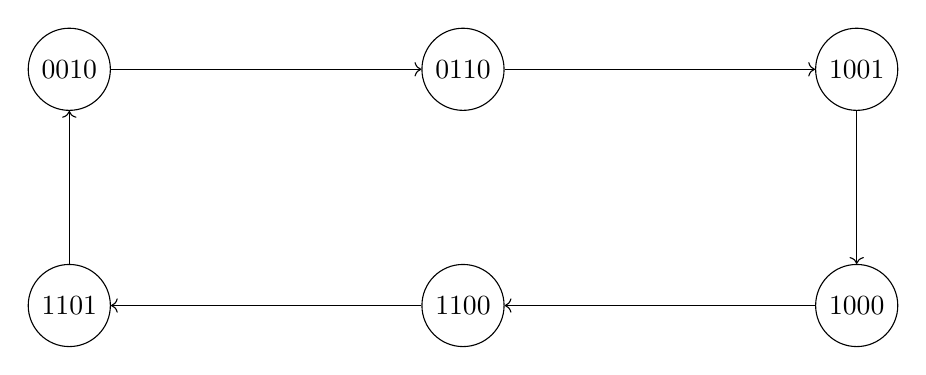
\begin{tikzpicture}[auto]
            \draw (0,0) node[state] (0010) {$0010$};
            \draw (5,0) node[state] (0110) {$0110$};
            \draw (10,0) node[state] (1001) {$1001$};
            \draw (0,-3) node[state] (1101) {$1101$};
            \draw (5,-3) node[state] (1100) {$1100$};
            \draw (10,-3) node[state] (1000) {$1000$};
            \path[->] (0010) edge (0110)
                      (0110) edge (1001)
                      (1001) edge (1000)
                      (1000) edge (1100)
                      (1100) edge (1101)
                      (1101) edge (0010);
        \end{tikzpicture}
    \end{figure}
    \newline and then we can derive the state table as follows
    \begin{table}[!htbp]
        \centering
    \begin{tabular}{p{.08\textwidth}<{\centering}p{.08\textwidth}<{\centering}p{.08\textwidth}<{\centering}p{.08\textwidth}<{\centering}
        p{.08\textwidth}<{\centering}p{.08\textwidth}<{\centering}p{.08\textwidth}<{\centering}p{.08\textwidth}<{\centering}}
        \toprule
        \multicolumn{4}{c}{\textbf{Present State}} & \multicolumn{4}{c}{\textbf{Next State}} \\
        \cmidrule(lr){1-4}\cmidrule(lr){5-8}
        $Q_3$ & $Q_2$ & $Q_1$ & $Q_0$ & $Q_3$ & $Q_2$ & $Q_1$ & $Q_0$ \\
        \midrule
        0 & 0 & 0 & 0 & 0 & 0 & 1 & 0 \\
        0 & 0 & 0 & 1 & 0 & 0 & 1 & 0 \\
        0 & 0 & 1 & 0 & 0 & 1 & 1 & 0 \\
        0 & 0 & 1 & 1 & 0 & 0 & 1 & 0 \\
        0 & 1 & 0 & 0 & 0 & 0 & 1 & 0 \\
        0 & 1 & 0 & 1 & 0 & 0 & 1 & 0 \\
        0 & 1 & 1 & 0 & 1 & 0 & 0 & 1 \\
        0 & 1 & 1 & 1 & 0 & 0 & 1 & 0 \\
        1 & 0 & 0 & 0 & 1 & 1 & 0 & 0 \\
        1 & 0 & 0 & 1 & 1 & 0 & 0 & 0 \\
        1 & 0 & 1 & 0 & 0 & 0 & 1 & 0 \\
        1 & 0 & 1 & 1 & 0 & 0 & 1 & 0 \\
        1 & 1 & 0 & 0 & 1 & 1 & 0 & 1 \\
        1 & 1 & 0 & 1 & 0 & 0 & 1 & 0 \\
        1 & 1 & 1 & 0 & 0 & 0 & 1 & 0 \\
        1 & 1 & 1 & 1 & 0 & 0 & 1 & 0 \\
        \bottomrule
    \end{tabular}
    \end{table}
    \newline And we can derive the Karnaugh maps for each DFF as follows
    \begin{figure}[!htbp]
        \centering
        \begin{karnaugh-map}(label=corner)[4][4][1][$Q_0$][$Q_1$][$Q_2$][$Q_3$]
            \minterms{6,8,9,12}
            \autoterms[0]
            \implicant{12}{8}
            \implicant{8}{9} 
            \implicant{6}{6}
        \end{karnaugh-map}
        \begin{karnaugh-map}(label=corner)[4][4][1][$Q_0$][$Q_1$][$Q_2$][$Q_3$]
            \minterms{2,8,12}
            \autoterms[0]
            \implicant{12}{8}
            \implicant{2}{2}
        \end{karnaugh-map}
        \begin{karnaugh-map}(label=corner)[4][4][1][$Q_0$][$Q_1$][$Q_2$][$Q_3$]
            \minterms{0,1,2,3,4,5,7,10,11,13,14,15}
            \autoterms[0]
            \implicant{0}{5}
            \implicant{0}{2}
            \implicant{5}{15}
            \implicant{15}{10}
        \end{karnaugh-map}
        \begin{karnaugh-map}(label=corner)[4][4][1][$Q_0$][$Q_1$][$Q_2$][$Q_3$]
            \minterms{6,12}
            \autoterms[0]
            \implicant{6}{6}
            \implicant{12}{12}
        \end{karnaugh-map}
    \end{figure}
    \newline so the simplified state equations for each DFF will be
    \begin{align*}
        Q_3(t+1) &= Q_3Q_1^{\prime}Q_0^{\prime} + Q_3Q_2^{\prime}Q_1^{\prime} + Q_3^{\prime}Q_2Q_1Q_0^{\prime} \\
        Q_2(t+1) &= Q_3Q_1^{\prime}Q_0^{\prime} + Q_3^{\prime}Q_2^{\prime}Q_1Q_0^{\prime} \\
        Q_1(t+1) &= Q_3^{\prime}Q_1^{\prime} + Q_2Q_0 + Q_3^{\prime}Q_2^{\prime} + Q_3Q_1 \\
        Q_0(t+1) &= Q_3^{\prime}Q_2Q_1Q_0^{\prime} + Q_3Q_2Q_1^{\prime}Q_0^{\prime}
    \end{align*}
    Since in DFF the excitation is equivelant to the state equation, we skip the input equations.
    To draw the logic diagram, we connect the input components based on the excitation to the D port of each DFF.
    \newline And the logic diagram will be like \newline
    \begin{figure}[!htbp]
        \centering
        \begin{circuitikz}[circuit logic IEC]
            \draw (1cm,0) node[d-ff1, rotate=90] (dff1) {};
            \draw (4cm,0) node[d-ff1, rotate=90] (dff2) {};
            \draw (7cm,0) node[d-ff1, rotate=90] (dff3) {};
            \draw (10cm,0) node[d-ff1, rotate=90] (dff4) {};
            \draw (1cm, -3cm) node[or port, number inputs=3, rotate=90] (or1) {};
            \draw (4cm, -3cm) node[or port, number inputs=2, rotate=90] (or2) {};
            \draw (7cm, -3cm) node[or port, number inputs=4, rotate=90] (or3) {};
            \draw (10cm, -3cm) node[or port, number inputs=2, rotate=90] (or4) {};
            \draw (0cm, -6cm) node[and port, rotate=90, number inputs=3] (and1) {};
            \draw (1.5cm, -6cm) node[and port, rotate=90, number inputs=3] (and2) {};
            \draw (3cm, -6cm) node[and port, rotate=90, number inputs=4] (and3) {};
            \draw (4.5cm, -6cm) node[and port, rotate=90, number inputs=4] (and4) {};
            \draw (6cm, -6cm) node[and port, rotate=90] (and5) {};
            \draw (7.5cm, -6cm) node[and port, rotate=90] (and6) {};
            \draw (9cm, -6cm) node[and port, rotate=90] (and7) {};
            \draw (10.5cm, -6cm) node[and port, rotate=90] (and8) {};
            \draw (12cm, -6cm) node[and port, rotate=90, number inputs=4] (and9) {};
            \draw (dff2.pin 3) -- ++(0,-0.5cm) node[fill=black,shape=circle,scale=0.3] (clkn1) {} ;
            \draw (dff3.pin 3) -- ++(0,-0.5cm) node[fill=black,shape=circle,scale=0.3] (clkn2) {} ;
            \draw (dff4.pin 3) -- ++(0,-0.5cm) node[fill=black,shape=circle,scale=0.3] (clkn3) {} ;
            \draw (dff1.pin 3) -- ++(0,-0.5cm) -- (clkn1) -- (clkn2) -- (clkn3) -- ++(.8cm,0) node[right] {$clk$};
            \draw (dff1.pin 6) -- ++(0,1.8cm) node[fill=black,shape=circle,scale=0.3] (q3) {} -- ++(0,0.7cm) node[above] {$Q_3$};
            \draw (dff2.pin 6) -- ++(0,1.6cm) node[fill=black,shape=circle,scale=0.3] (q2) {} -- ++(0,0.9cm) node[above] {$Q_2$};
            \draw (dff3.pin 6) -- ++(0,1.4cm) node[fill=black,shape=circle,scale=0.3] (q1) {} -- ++(0,1.1cm) node[above] {$Q_1$};
            \draw (dff4.pin 6) -- ++(0,1.2cm) node[fill=black,shape=circle,scale=0.3] (q0) {} -- ++(0,1.3cm) node[above] {$Q_0$};
            \draw (dff1.pin 4) -- ++(0,1cm) -- ++(11.6cm,0) -- ++(0,-11cm) -| (and3.in 1);
            \draw (dff2.pin 4) -- ++(0,0.8cm) -- ++(8.4cm,0) -- ++(0,-10.6cm) -| (and4.in 2);
            \draw (dff3.pin 4) -- ++(0,0.6cm) -- ++(5.2cm,0) -- ++(0,-10.2cm) -| (and1.in 3) ;
            \draw (dff4.pin 4) -- ++(0,0.4cm) -- ++(2cm,0) -- ++(0,-9.8cm) -| (and3.in 4) ;
            \draw (or1.out) -| (dff1.pin 1) (or2.out) -| (dff2.pin 1) (or3.out) -| (dff3.pin 1) (or4.out) -| (dff4.pin 1);
            \draw (and1.out) |- (or1.in 1) (and2.out) -- ++ (0,17pt) node[fill=black,shape=circle,scale=0.3]{} -| (or1.in 2) (and2.out) -- ++ (0,17pt) -| (or2.in 1);
            \draw (and3.out) |- (or1.in 3) (and3.out) -- ++(0,9pt) node[fill=black,shape=circle,scale=0.3]{} -| (or4.in 1);
            \draw (and4.out) -| (or2.in 2) (and5.out) |- (or3.in 1) (and6.out) -| (or3.in 2)
                  (and7.out)  -- ++(0,4pt) -| (or3.in 3) (and8.out) -- ++(0,15pt) -| (or3.in 4)
                  (and9.out) |- (or4.in 2);
            \draw (q3) -- ++(-45pt,0) -- ++(0,-11cm) -| (and9.in 1);
            \draw (q2) -- ++(-2.8cm,0) -- ++(-45pt,0) -- ++(0,-10.6cm) -| (and3.in 2);
            \draw (q1) -- ++(-5.6cm,0) -- ++(-45pt,0) -- ++(0,-10.2cm) -| (and4.in 3);
            \draw (q0) -- ++(-8.4cm,0) -- ++(-45pt,0) -- ++(0,-9.8cm) -| (and9.in 4);
            \draw (and1.in 1) -- ++(0,-1cm) node[fill=black,shape=circle,scale=0.3]{}
                  (and1.in 2) -- ++(0,-0.8cm) node[fill=black,shape=circle,scale=0.3]{};
            \draw (and2.in 1) -- ++(0,-1cm) node[fill=black,shape=circle,scale=0.3]{}
                  (and2.in 2) -- ++(0,-1.4cm) node[fill=black,shape=circle,scale=0.3]{}
                  (and2.in 3) -- ++(0,-0.4cm) node[fill=black,shape=circle,scale=0.3]{};
            \draw (and3.in 3) -- ++(0,-0.6cm) node[fill=black,shape=circle,scale=0.3]{};
            \draw (and4.in 1) -- ++(0,-1.8cm) node[fill=black,shape=circle,scale=0.3]{}
                  (and4.in 4) -- ++(0,-1.2cm) node[fill=black,shape=circle,scale=0.3]{};
            \draw (and5.in 1) -- ++(0,-1.6cm) node[fill=black,shape=circle,scale=0.3]{}
                  (and5.in 2) -- ++(0,-1.2cm) node[fill=black,shape=circle,scale=0.3]{};
            \draw (and6.in 1) -- ++(0,-1.8cm) node[fill=black,shape=circle,scale=0.3]{}
                  (and6.in 2) -- ++(0,-1.4cm) node[fill=black,shape=circle,scale=0.3]{};
            \draw (and7.in 1) -- ++(0,-1.8cm) node[fill=black,shape=circle,scale=0.3]{}
                  (and7.in 2) -- ++(0,-0.4cm) node[fill=black,shape=circle,scale=0.3]{};
            \draw (and8.in 1) -- ++(0,-1.8cm) node[fill=black,shape=circle,scale=0.3]{}
                  (and8.in 2) -- ++(0,-1.6cm) node[fill=black,shape=circle,scale=0.3]{};
            \draw (and9.in 2) -- ++(0,-1.6cm) node[fill=black,shape=circle,scale=0.3]{}
                  (and9.in 3) -- ++(0,-1.4cm) node[fill=black,shape=circle,scale=0.3]{};
        \end{circuitikz}
    \end{figure}
\end{solution}

\begin{problem}
    Design a counter with T flip-flops that goes through the following binary repeated
    sequence: 0, 1, 3, 7, 6, 4. Derive the input equations for the FFs. Show that when binary
    states 010 and 101 are considered as don't care conditions, the counter may not operate
    properly.
\end{problem}

\begin{solution}
    From the sequence, we can derive the state diagram as follows.
    \begin{figure}[!htbp]
        \centering
        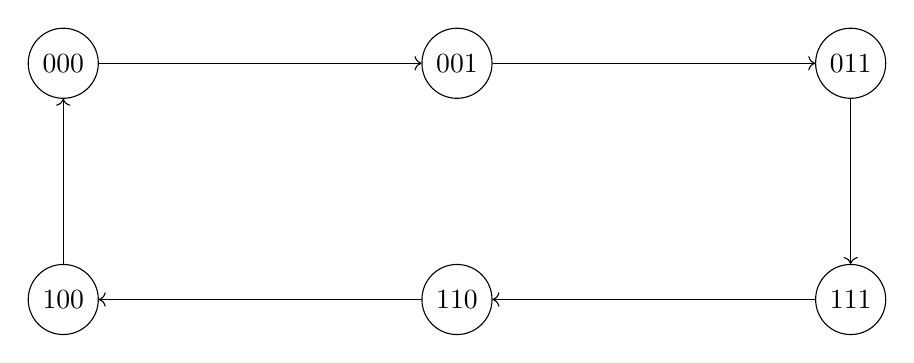
\begin{tikzpicture}[auto]
            \draw (0,0) node[state] (000) {$000$};
            \draw (5,0) node[state] (001) {$001$};
            \draw (10,0) node[state] (011) {$011$};
            \draw (10,-3) node[state] (111) {$111$};
            \draw (5,-3) node[state] (110) {$110$};
            \draw (0,-3) node[state] (100) {$100$};
            \path[->] (000) edge (001)
                      (001) edge (011)
                      (011) edge (111)
                      (111) edge (110)
                      (110) edge (100)
                      (100) edge (000);
        \end{tikzpicture}
    \end{figure}
    \newline and then we can derive the state table as follows
    \begin{table}[!htbp]
        \centering
    \begin{tabular}{p{.07\textwidth}<{\centering}p{.07\textwidth}<{\centering}p{.07\textwidth}<{\centering}p{.07\textwidth}<{\centering}
        p{.07\textwidth}<{\centering}p{.07\textwidth}<{\centering}p{.07\textwidth}<{\centering}p{.07\textwidth}<{\centering}p{.07\textwidth}<{\centering}}
        \toprule
        \multicolumn{3}{c}{\textbf{Present State}} & \multicolumn{3}{c}{\textbf{Next State}}& \multicolumn{3}{c}{\textbf{JKFF Inputs}} \\
        \cmidrule(lr){1-3}\cmidrule(lr){4-6}\cmidrule(lr){7-9}
        $Q_2$ & $Q_1$ & $Q_0$ & $Q_2$ & $Q_1$ & $Q_0$ & $T_2$ & $T_1$ & $T_0$ \\
        \midrule
        0 & 0 & 0 & 0 & 0 & 1 & 0 & 0 & 1 \\
        0 & 0 & 1 & 0 & 1 & 1 & 0 & 1 & 0 \\
        0 & 1 & 0 & X & X & X & X & X & X \\
        0 & 1 & 1 & 1 & 1 & 1 & 1 & 0 & 0 \\
        1 & 0 & 0 & 0 & 0 & 0 & 1 & 0 & 0 \\
        1 & 0 & 1 & X & X & X & X & X & X \\
        1 & 1 & 0 & 1 & 0 & 0 & 0 & 1 & 0 \\
        1 & 1 & 1 & 1 & 1 & 0 & 0 & 0 & 1 \\
        \bottomrule
    \end{tabular}
    \end{table}
    \newline And we can derive the Karnaugh maps for each TFF as follows
    \begin{figure}[!htbp]
        \centering
        \begin{karnaugh-map}(label=corner)[4][2][1][$Q_0$][$Q_1$][$Q_2$]
            \minterms{3,4}
            \terms{2,5}{X}
            \autoterms[0]
            \implicant{3}{2}
            \implicant{4}{5}
        \end{karnaugh-map}
        \begin{karnaugh-map}(label=corner)[4][2][1][$Q_0$][$Q_1$][$Q_2$]
            \minterms{1,6}
            \terms{2,5}{X}
            \autoterms[0]
            \implicant{1}{5}
            \implicant{2}{6}
        \end{karnaugh-map}
    \end{figure}
    \begin{figure}[!htbp]
        \centering
        \begin{karnaugh-map}(label=corner)[4][2][1][$Q_0$][$Q_1$][$Q_2$]
            \minterms{0,7}
            \terms{2,5}{X}
            \autoterms[0]
            \implicant{5}{7}
            \implicantedge{0}{0}{2}{2}
        \end{karnaugh-map}
    \end{figure}
    \newline If we count the don't care conditions, the simplified input equation will be
    \begin{align*}
        Q_2(t+1) &= Q_2Q_1^{\prime} + Q_2^{\prime}Q_1 = Q_2\oplus Q_1 \\
        Q_1(t+1) &= Q_1Q_0^{\prime} + Q_1Q_0^{\prime} = Q_1\oplus Q_0 \\
        Q_0(t+1) &= Q_2Q_0 + Q_2^{\prime}Q_0^{\prime} = (Q_2\oplus Q_0)^{\prime}
    \end{align*}
    and the state table will be turned into
    \begin{table}[!htbp]
        \centering
    \begin{tabular}{p{.07\textwidth}<{\centering}p{.07\textwidth}<{\centering}p{.07\textwidth}<{\centering}p{.07\textwidth}<{\centering}
        p{.07\textwidth}<{\centering}p{.07\textwidth}<{\centering}p{.07\textwidth}<{\centering}p{.07\textwidth}<{\centering}p{.07\textwidth}<{\centering}}
        \toprule
        \multicolumn{3}{c}{\textbf{Present State}} & \multicolumn{3}{c}{\textbf{Next State}}& \multicolumn{3}{c}{\textbf{JKFF Inputs}} \\
        \cmidrule(lr){1-3}\cmidrule(lr){4-6}\cmidrule(lr){7-9}
        $Q_2$ & $Q_1$ & $Q_0$ & $Q_2$ & $Q_1$ & $Q_0$ & $T_2$ & $T_1$ & $T_0$ \\
        \midrule
        0 & 0 & 0 & 0 & 0 & 1 & 0 & 0 & 1 \\
        0 & 0 & 1 & 0 & 1 & 1 & 0 & 1 & 0 \\
        0 & 1 & 0 & 1 & 0 & 1 & 1 & 1 & 1 \\
        0 & 1 & 1 & 1 & 1 & 1 & 1 & 0 & 0 \\
        1 & 0 & 0 & 0 & 0 & 0 & 1 & 0 & 0 \\
        1 & 0 & 1 & 0 & 1 & 0 & 1 & 1 & 1 \\
        1 & 1 & 0 & 1 & 0 & 0 & 0 & 1 & 0 \\
        1 & 1 & 1 & 1 & 1 & 0 & 0 & 0 & 1 \\
        \bottomrule
    \end{tabular}
    \end{table}
    \newline From the state table we could see clearly that if we treat 010 and 101 as don't care condition,
    the counter will be trapped in a infinite loop between 010 and 101 when we encounter either of the states.
    Therefore we shall assign 011 to the next state of state 010, and 110 to that of 101 to enable the counter with self-correction.
    So the state table, Kmaps and simplified equation will be
    \begin{table}[!htbp]
        \centering
    \begin{tabular}{p{.07\textwidth}<{\centering}p{.07\textwidth}<{\centering}p{.07\textwidth}<{\centering}p{.07\textwidth}<{\centering}
        p{.07\textwidth}<{\centering}p{.07\textwidth}<{\centering}p{.07\textwidth}<{\centering}p{.07\textwidth}<{\centering}p{.07\textwidth}<{\centering}}
        \toprule
        \multicolumn{3}{c}{\textbf{Present State}} & \multicolumn{3}{c}{\textbf{Next State}}& \multicolumn{3}{c}{\textbf{JKFF Inputs}} \\
        \cmidrule(lr){1-3}\cmidrule(lr){4-6}\cmidrule(lr){7-9}
        $Q_2$ & $Q_1$ & $Q_0$ & $Q_2$ & $Q_1$ & $Q_0$ & $T_2$ & $T_1$ & $T_0$ \\
        \midrule
        0 & 0 & 0 & 0 & 0 & 1 & 0 & 0 & 1 \\
        0 & 0 & 1 & 0 & 1 & 1 & 0 & 1 & 0 \\
        0 & 1 & 0 & 0 & 1 & 1 & 0 & 0 & 1 \\
        0 & 1 & 1 & 1 & 1 & 1 & 1 & 0 & 0 \\
        1 & 0 & 0 & 0 & 0 & 0 & 1 & 0 & 0 \\
        1 & 0 & 1 & 1 & 1 & 0 & 0 & 1 & 1 \\
        1 & 1 & 0 & 1 & 0 & 0 & 0 & 1 & 0 \\
        1 & 1 & 1 & 1 & 1 & 0 & 0 & 0 & 1 \\
        \bottomrule
    \end{tabular}
    \end{table}
    \begin{figure}[!htbp]
        \centering
        \begin{karnaugh-map}(label=corner)[4][2][1][$Q_0$][$Q_1$][$Q_2$]
            \minterms{3,4}
            \autoterms[0]
            \implicant{3}{3}
            \implicant{4}{4}
        \end{karnaugh-map}
        \begin{karnaugh-map}(label=corner)[4][2][1][$Q_0$][$Q_1$][$Q_2$]
            \minterms{1,5,6}
            \autoterms[0]
            \implicant{1}{5}
            \implicant{6}{6}
        \end{karnaugh-map}
        \begin{karnaugh-map}(label=corner)[4][2][1][$Q_0$][$Q_1$][$Q_2$]
            \minterms{0,2,5,7}
            \autoterms[0]
            \implicant{5}{7}
            \implicantedge{0}{0}{2}{2}
        \end{karnaugh-map}
    \end{figure}
    \begin{align*}
        Q_2(t+1) &= Q_2Q_1^{\prime}Q_0^{\prime} + Q_2^{\prime}Q_1Q_0 \\
        Q_1(t+1) &= Q_1^{\prime}Q_0 + Q_2Q_1Q_0^{\prime}
    \end{align*}
    \[ Q_0(t+1) = Q_2Q_0 + Q_2^{\prime}Q_0^{\prime} = (Q_2\oplus Q_0)^{\prime} \]
    and finally we can draw the logic diagram based on the equations
    \begin{figure}[!htbp]
        \centering
        \setlength{\belowcaptionskip}{+0.4cm}
        \begin{circuitikz}[circuit logic IEC]
            \draw (0,0) node[t-ff, rotate=90] (tff1) {};
            \draw (4cm,0) node[t-ff, rotate=90] (tff2) {};
            \draw (8cm,0) node[t-ff, rotate=90] (tff3) {};
            \draw ([yshift=-2cm]tff1.pin 3) node[or port, rotate=90] (or1) {} (or1.out) -- (tff1.pin 3);
            \draw ([yshift=-2cm]tff2.pin 3) node[or port, rotate=90] (or2) {} (or2.out) -- (tff2.pin 3);
            \draw ([yshift=-2cm]tff3.pin 3) node[xnor port, rotate=90] (or3) {} (or3.out) -- (tff3.pin 3);
            \draw (-0.3cm,-6cm) node[and port, rotate=90, number inputs=3] (and1) {};
            \draw (2cm,-6cm) node[and port, rotate=90, number inputs=3] (and2) {};
            \draw (4cm,-6cm) node[and port, rotate=90] (and3) {};
            \draw (6cm,-6cm) node[and port, rotate=90, number inputs=3] (and4) {};
            \draw (and1.out) |- (or1.in 1) (and2.out) |- (or1.in 2) (and3.out) |- (or2.in 1) (and4.out) |- (or2.in 2);
            \draw (tff1.pin 4) -- ++(0,0.8cm) node[fill=black,shape=circle,scale=0.3] (q2) {} -- ++(0,1cm) node[above] {$Q_2$};
            \draw (tff2.pin 4) -- ++(0,0.6cm) node[fill=black,shape=circle,scale=0.3] (q1) {} -- ++(0,1.2cm) node[above] {$Q_1$};
            \draw (tff3.pin 4) -- ++(0,0.4cm) node[fill=black,shape=circle,scale=0.3] (q0) {} -- ++(0,1.4cm) node[above] {$Q_0$};
            \draw (tff2.pin 1) -- ++(0,-0.5cm) node[fill=black,shape=circle,scale=0.3] (clkn2) {} ;
            \draw (tff3.pin 1) -- ++(0,-0.5cm) node[fill=black,shape=circle,scale=0.3] (clkn3) {} ;
            \draw (tff1.pin 1) -- ++(0,-0.5cm) -- (clkn2) -- (clkn3) -- ++(2cm,0) node[right] {$clk$};
            \draw (q2) -- ++(-3.5cm,0) -- ++(0,-10cm) -| (or3.in 2);
            \draw (q1) -- ++(-7.3cm,0) -- ++(0,-9.6cm) -| (and4.in 2);
            \draw (q0) -- ++(-11.1cm,0) -- ++(0,-9.2cm) -| (or3.in 1);
            \draw (and1.in 1) -- ++(0,-1cm) node[fill=black,shape=circle,scale=0.3]{}
                  (and1.in 2) -- ++(0,-0.8cm) node[fill=black,shape=circle,scale=0.3]{}
                  (and1.in 2) -- ++(0,0.3cm) node[notcirc] {}
                  (and1.in 3) -- ++(0,-0.6cm) node[fill=black,shape=circle,scale=0.3]{}
                  (and1.in 3) -- ++(0,0.3cm) node[notcirc] {};
            \draw (and2.in 1) -- ++(0,-1cm) node[fill=black,shape=circle,scale=0.3]{}
                  (and2.in 2) -- ++(0,-0.8cm) node[fill=black,shape=circle,scale=0.3]{}
                  (and2.in 1) -- ++(0,0.3cm) node[notcirc] {}
                  (and2.in 3) -- ++(0,-0.6cm) node[fill=black,shape=circle,scale=0.3]{};
            \draw (and3.in 1) -- ++(0,-0.8cm) node[fill=black,shape=circle,scale=0.3]{}
                  (and3.in 2) -- ++(0,-0.6cm) node[fill=black,shape=circle,scale=0.3]{}
                  (and3.in 1) -- ++(0,0.3cm) node[notcirc] {};
            \draw (and4.in 1) -- ++(0,-1cm) node[fill=black,shape=circle,scale=0.3]{}
                  (and4.in 3) -- ++(0,0.3cm) node[notcirc] {}
                  (and4.in 3) -- ++(0,-0.6cm) node[fill=black,shape=circle,scale=0.3]{};
        \end{circuitikz}
    \end{figure}
\end{solution}

\end{document}